%!TEX root = ../main.tex

The results of this thesis are intended to show evidence of a working system, and in particular the performance of subsystems. The validation and explanation of such subsystems is vital to the validity of the work done in this thesis. 
\section{Cost of Block}
In the implementation of this thesis three methods were selected to represent the cost of a block, from these three the Mixed integer linear program with validity constraints was selected to be the model used in the final iteration of the project. The model was then compared to the results generated by preexisting algorithms\cite{A*Search} such that a validation could be made, the comparison of these two methods is seen below in table \ref{tableres}. 

\begin{center}
% \caption{Validation of results}
\label{tableres}
 \begin{tabular}{|c| c| c|c|} 
 \hline
 Length of Block & Operation Cost& True Cost & Error (\%)\\ 
 32 & 7466 & 7377 & 1.206\\ 
 \hline
 37 & 8578 & 8383 & 2.326 \\
 \hline
 42 & 9743 & 9314 & 4.606 \\
 \hline
 47 & 10908 & 10229 & 6.638 \\
 \hline
 52 & 12020 & 11554 & 4.033\\ 
 \hline
\end{tabular}
\end{center}



As table \ref{tableres} shows the error between the true values and the calculated values increases as the length of the block increases, this could be in part due to differences and assumptions made in the modeling of the spoil channel and spoil capacity. However it is also reasonable that this error is due in no small part to the assumptions made when reducing a three dimensional problem into two dimensions an as such could be seen as a potential validation of the model of block costing, furthermore the typical cost of a block for any environment seems to have similar results through all blocks, with the more complex datasets (5,6,7,8,9,10) having a larger cost in general than the simpler counterparts. As seen in table \ref{RESMIP} the results for sets 1,3,4,5 were all very similar, however the results for the more complex blocks are often larger as the range of feasible solutions is lower. This suggests that the cost of a block is dependent on location, length and spoil, and as such methods such as machine learning or linear simplifications may not be valid. 
\begin{center}
\begin{tabular}{ | c | c | c | c | c | c |}
\hline
\label{RESMIP}
% \caption{Compilation of results}
	% \hline
	Length & Set 1 & Set 2 & Set 3 & Set 4 & Set 5  \\ \hline
	32 & 7466.6 & 5772.1 & 7201.9 & 7784.4 & 7466.6  \\ \hline
	37 & 8578.7 & 6884.1 & 8261 & 9108.2 & 8472.8  \\ \hline
	42 & 9743.7 & 8419.8 & 9055.3 & 10696.9 & 9214.1 \\ \hline
	47 & 10908.7 & 10008.5 & 10114.4 & 12285.5 & 10008.5 \\ \hline
	52 & 12020.7 & 10855.7 & 11173.5 & 13768.3 & 11226.4 \\ \hline
	\hline
	Length & Set 6 & Set 7 & Set 8 & Set 9 & Set 10  \\ \hline
	32 & 7625.5 & 8261 & 7519.6 & 7360.7 & 9002.3  \\ \hline
	37& 8737.5 & 9320 & 8525.7& 8261 & 10326.2  \\ \hline
	42 & 10061.4 & 10485.1 & 9373 & 9214.1 & 11491.2 \\ \hline
	47 & 11173.5 & 12073.7 & 10167.3 & 9743.7& 12020.7 \\ \hline
	52 & 12020.7 & 13079.8 & 10961.6 & 11120.5 & 12762.1  \\ \hline

	 % &  &  &  &  &  &  &  &  &  &  & \  & \  \\ \hline
\end{tabular}
\end{center}
However the cost of a block is not the only output generated by the model, the state of the spoil after the block has been removed is also returned. Spoil constraints on the overall solution require accurate and appropriate spoil functions to be generated, as seen in figure \ref{MIPDemo1} the spoil of a block is simply calculated and returned as an array of capacities. These results would suggest that typically overburden is deposited as close to the current block as possible, this is due to the reduced cost associated with smaller movements , the only variation to this heuristic is when nearby spoil sections are at capacity, this situation will often generate more interesting blocks  as the constraint on the spoil will limit the movement and motion of the dragline. The spoil shown in figure \ref{MIPDemo2} is an indication of how the spoil interacts when a sequence of blocks is taken, the initial block will have a wider range of spoil sections and the second block must deposit overburden closer to the capacity of sections, if the capacity of a section is close to its limit then the secondary block may have to add overburden to previously used spoil sections, which while not efficient will still resolve in a feasible solution. 

\begin{figure}[h]
\caption{Resultant spoil of a Block}
\label{MIPDemo1}
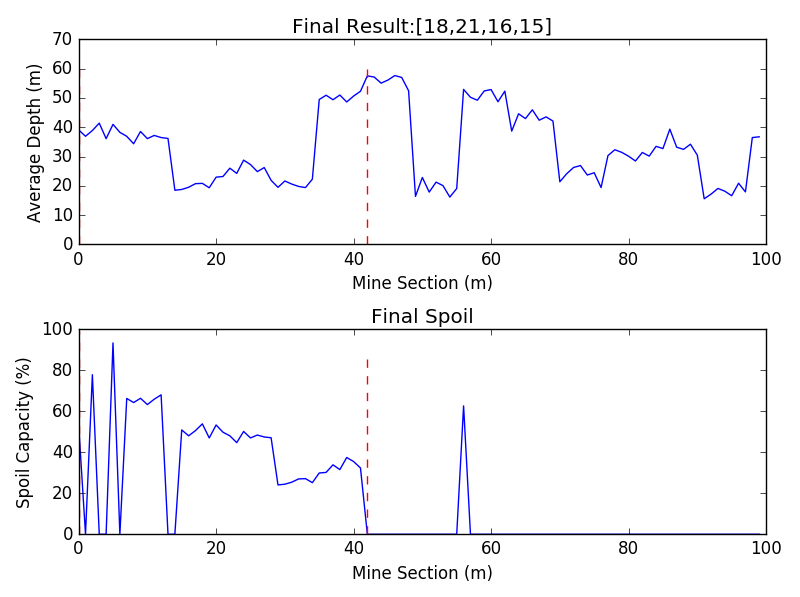
\includegraphics[width=\textwidth]{MIP_Demo1.png}
\end{figure}

\begin{figure}[h]
\caption{Resultant spoil of a second Block}
\label{MIPDemo2}
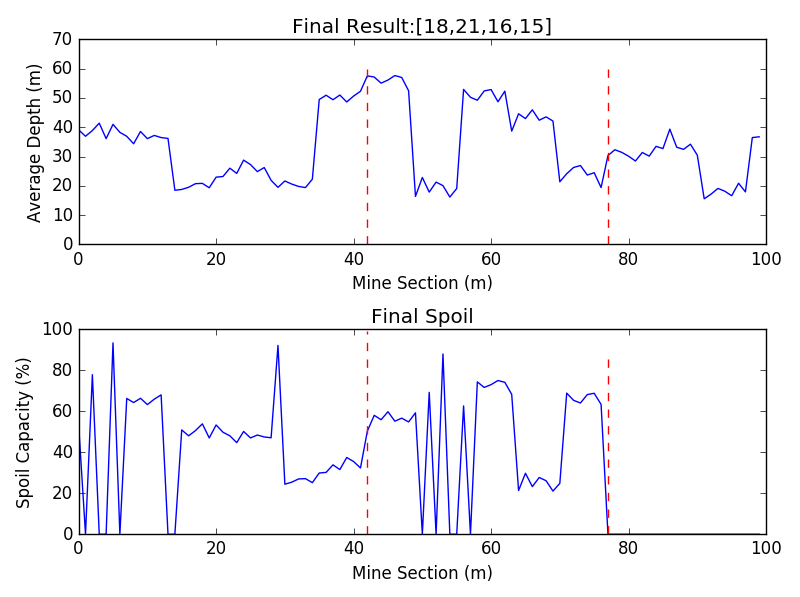
\includegraphics[width=\textwidth]{MIP_Demo2.png}
\end{figure}

\section{Strip Planning}
The sequence generation of potential solutions is the key component to solving the optimisation of a strip, this method reduces the problem space dramatically and is used to ensure that only potentially valid solutions are considered. However the complexity of such an operation is $O(2^n)$ and as such for much larger strips a lower resolution may need to be considered. In the below table is an example of the amount of valid solutions compared to invalid solutions for a variety of strips that were tested upon.
\begin{center}
\label{tableres2}
 \begin{tabular}{|c| c| c|c|c|c|} 
 \hline
 Length of Strip &  Range & Resolution & Raw Solutions & Valid Solutions & Time Taken\\ 
 70 & (15,35) & 1m & $10^5$ & 574 & 0.4s\\ 
 \hline
 100 & (15,35) & 1m & $10^9$ & 31393 & 11.2s\\
 \hline
 100 & (15,35)& 5m & $10^9$ & 153 & 0.2s\\
 \hline
 500 & (30,65)& 1m & $10^16$ & $10^9$ & 900s\\
 \hline
 500 & (30,65) & 5m & $10^16$ &$10^8$ & 500s \\ 
 \hline
 500 & (30,65) & 10m & $10^16$& $10^6$ & 100s\\ 
 \hline
\end{tabular}
\end{center}
 The results in \ref{tableres2} show that despite the exponential complexity the solution to the sequence generation can still be calculated in reasonable time with dramatic reductions in solutions explored. This time saving allows the dynamic program to rapidly calculate optimal solutions, the use of memotisation also reduces the function calls dramatically as the set of feasible sequences is ordered and each element is unique. In the below table the optimal solutions for each method are supplied, with the appropriate metrics, these methods can then be compared to the standard methods used in mining.
 \begin{center} 
  \begin{tabular}{|c| c| c|c|c|} 
 \hline
 Length of Strip & Blocksize Range & Resolution & Optimal Sequence & Time Taken\\ 
 70 & (15,35) & 1m  & 18,21,16,15 & 240s\\ 
 \hline
 100 & (15,35) & 1m  & 19,18,24,23,16 & 10464s\\
 \hline
 100 & (15,35)& 5m  & 20,25,25,25,15 & 70s\\
 \hline
 500 & (30,65)& 1m & ---& Timeout\\
 \hline
 500 & (30,65) & 5m  &--- & Timeout \\ 
 \hline
 500 & (30,65) & 10m &  60,60,60,50,50,50,& \\
 & & & 40,40,30,30,30 & 32000s\\ 
 \hline
\end{tabular}
\end{center}
These results suggest that the optimal solution tends to typically utilize longer blocks initially however will use shorter blocks as the spoil becomes more complex, this is intuitively simple and could be used as a heuristic to further reduce the solution space considered. However this is different to the methods commonly used in mining\cite{IntoOpenPit} which suggests a consistent block length regardless of the topology of the mine. This does not agree with the methods and results supplied by the algorithms created and suggests room for improvement in the optimisation of strip mining. Furthermore the algorithms inability to solve and optimise for a strip is due to the still colossal range of solutions that are available for such a problem, while simplifications and lower resolutions will be able to generate feasible solutions with reasonable characteristics. However for future adaptation of this code it could be considered to use stronger admissible heuristics to reduce the run time of an operation\\An alternate solution is that  the strip of a mine could be treated as a series of sub strips which all must be solved feasibly before the overall sequencing  of the total strip is  done, that is if a strip is 700m long, it could be modeled as ten 70m long strips with the additional constraint that the spoils of each sub strip is independent. This method was implemented as it is simple to test and was found that breaking a strop into smaller substrips generated feasible solutions that are optimal for each sub strip. While this will not be optimal for the mine overall it will allow solutions that perform well to be found quickly, rather than truly optimal solutions which could take days to calculate. 


